%%%%%%%%%%%%%%%%%%%%%%%%%%%%%%%%%%%%%%%%%
% Programming/Coding Assignment
% LaTeX Template
%
% This template has been downloaded from:
% http://www.latextemplates.com
%
% Original author:
% Ted Pavlic (http://www.tedpavlic.com)
%
% Note:
% The \lipsum[#] commands throughout this template generate dummy text
% to fill the template out. These commands should all be removed when 
% writing assignment content.
%
% This template uses a Perl script as an example snippet of code, most other
% languages are also usable. Configure them in the "CODE INCLUSION 
% CONFIGURATION" section.
%
%%%%%%%%%%%%%%%%%%%%%%%%%%%%%%%%%%%%%%%%%

%----------------------------------------------------------------------------------------
%	PACKAGES AND OTHER DOCUMENT CONFIGURATIONS
%----------------------------------------------------------------------------------------

\documentclass[11pt]{article}

\usepackage{fancyhdr} % Required for custom headers
\usepackage{lastpage} % Required to determine the last page for the footer
\usepackage{extramarks} % Required for headers and footers
\usepackage[usenames,dvipsnames]{color} % Required for custom colors
\usepackage{graphicx} % Required to insert images
\usepackage{listings} % Required for insertion of code
\usepackage{courier} % Required for the courier font
\usepackage{lipsum} % Used for inserting dummy 'Lorem ipsum' text into the template
\usepackage{amssymb}
\usepackage{amsmath}
\usepackage{amsthm}
\usepackage[utf8]{inputenc}
\usepackage{float}
\usepackage{geometry}
\usepackage{tikz}
\usepackage{changepage}
\usepackage{float}
\usetikzlibrary{positioning}
\geometry{
letterpaper,
top=1.5in,
bottom=1.5in,
left=1.5in,
right=1.5in
}

\newcommand{\R}{\mathbb{R}}
\newcommand{\N}{\mathbb{N}}
\newcommand{\Z}{\mathbb{Z}}
\newcommand{\e}{\epsilon}
\renewcommand{\d}{\delta}
\renewcommand{\a}{\alpha}
\renewcommand{\b}{\beta}


\linespread{1.1} % Line spacing
\setlength{\parskip}{1em}
\setlength\parindent{0pt} % Removes all indentation from paragraphs

%----------------------------------------------------------------------------------------
%	CODE INCLUSION CONFIGURATION
%----------------------------------------------------------------------------------------

\definecolor{MyDarkGreen}{rgb}{0.0,0.4,0.0} % This is the color used for comments
\lstloadlanguages{Python} % Load Perl syntax for listings, for a list of other languages supported see: ftp://ftp.tex.ac.uk/tex-archive/macros/latex/contrib/listings/listings.pdf
\lstset{language=Python, % Use Perl in this example
	 breaklines=true,
	 postbreak=\mbox{\textcolor{red}{$\hookrightarrow$}\space},
        frame=single, % Single frame around code
        basicstyle=\small\ttfamily, % Use small true type font
        keywordstyle=[1]\color{Blue}\bf, % Perl functions bold and blue
        keywordstyle=[2]\color{Purple}, % Perl function arguments purple
        keywordstyle=[3]\color{Blue}\underbar, % Custom functions underlined and blue
        identifierstyle=, % Nothing special about identifiers                                         
        commentstyle=\usefont{T1}{pcr}{m}{sl}\color{MyDarkGreen}\small, % Comments small dark green courier font
        stringstyle=\color{Purple}, % Strings are purple
        showstringspaces=false, % Don't put marks in string spaces
        tabsize=5, % 5 spaces per tab
        %
        % Put standard Perl functions not included in the default language here
        morekeywords={rand},
        %
        % Put Perl function parameters here
        morekeywords=[2]{on, off, interp},
        %
        % Put user defined functions here
        morekeywords=[3]{test},
       	%
        morecomment=[l][\color{Blue}]{...}, % Line continuation (...) like blue comment
        numbers=left, % Line numbers on left
        firstnumber=1, % Line numbers start with line 1
        numberstyle=\tiny\color{Blue}, % Line numbers are blue and small
        stepnumber=5 % Line numbers go in steps of 5
}




%----------------------------------------------------------------------------------------
%	NAME AND CLASS SECTION
%----------------------------------------------------------------------------------------

\newcommand{\hmwkTitle}{\\Final Project\vspace{0.5cm}} % Assignment title
\newcommand{\hmwkDueDate}{Wednesday,\ December\ 13,\ 2017} % Due date
\newcommand{\hmwkClass}{Neural Networks, CS\ 6890/ECE\ 5930} % Course/class
\newcommand{\hmwkClassTime}{MWF @ 2:30 PM} % Class/lecture time
\newcommand{\hmwkClassInstructor}{Todd Moon} % Teacher/lecturer
\newcommand{\hmwkAuthorName}{Hans Gunther, Sam Schwartz, Tyler Bowles} % Your name

%----------------------------------------------------------------------------------------
%	TITLE PAGE
%----------------------------------------------------------------------------------------

\title{
\vspace{2in}
\textmd{\textbf{\hmwkClass:\ \hmwkTitle}}\\
\normalsize\vspace{0.1in}\small{Due\ on\ \hmwkDueDate}\\
\vspace{0.1in}\large{\textit{\hmwkClassInstructor\, \hmwkClassTime}}
\vspace{3in}
}

\author{\textbf{\hmwkAuthorName}}
\date{} % Insert date here if you want it to appear below your name

%----------------------------------------------------------------------------------------

\begin{document}

\maketitle

%----------------------------------------------------------------------------------------
%	TABLE OF CONTENTS
%----------------------------------------------------------------------------------------

%\setcounter{tocdepth}{1} % Uncomment this line if you don't want subsections listed in the ToC

\newpage
\tableofcontents
\newpage



\section{Introduction}

\textit{(This section satisfies Expectation 1)}

Dear Dr. Moon,

In English 1010 we allegedly learn to write to a target audience. In this case, that target audience is, well, you. Excuse the narrative approach of this report if it wasn’t expected, but who doesn’t love a personalized letter right before The Holidays? 

It goes without saying that we would have loved to have tinkered on this project for longer; most interesting projects tend to bleed out greater than the length of a semester, and this was an interesting project indeed.

With that said, we have a working network structure and are proud of the results given the time we had. We hope to intrigue you along the way, detailing our thought process and results of that thought process. We’ve learned a lot from this experience, and we’ve learned a lot from you. Thank you.

The rest of this report is divvied out into sections roughly parallelizing the expectations outlined in the Canvas message sent on Monday, December 11. Namely, the architecture of our setup, the training process, the overall accuracy, and final remarks. The code is attached to the end as an appendix. In each section, we’ve striven to not only express the “what” of our decisions, but the rationale behind them.

We hope you enjoy the rest of this document.

\hfill
\parbox{5cm}{
\vspace{1.5cm}
With excited anticipation,\\[1.5cm]
Hans, Sam, and Tyler\\[1cm]
}

\newpage






\newpage\section{Architecture}
\textit{(This section satisfies Expectations 2 and 3)}

\begin{quote}
\centering
``Simplicity is prerequisite for reliability.'' - Edsger Dijkstra
\end{quote}

\subsection{High Level Technical Overview}

In order to train any sort of network structure, we wanted to partition the input data from each channel into short, fixed segments of length $n$ milliseconds. We affectionately call these segments ``chunks''. Since there are two channels, each chunk could be viewed as a $2\times (n\cdot s)$ matrix, where $s$ is the sampling-rate of the audio file in question. In the event of an input file not being exactly divisible by $n$ milliseconds, the final chunk of the file was padded with zeros so that all chunks were of equal length.

All chunks were then given a classification represented by $2\times 1$ matrices, indicating whether or not there was speech present in each channel of the chunk. The goal of the neural network would be to assign two boolean values to newly seen chunks of length $2\times (n\cdot s)$ indicating whether there was human speech in the corresponding channel.

Once each of the $k$ chunks in an audio file was classified, the resultant boolean outcomes would be joined into a $2\times k$ matrix sent to a post-processing script to do any final data smoothing and write the classification to CSV files in the format provided by Dr. Borrie.

In short, the psuedo-code for an end user of our software looks like this:

\begin{minipage}{\linewidth}
\begin{lstlisting}[language=Python]
audiofile = open_audio_file(filename)
chunks[] = divide_audio_file_into_chunks(chunk_length=100ms)
outputs = []
for chunk in chunks:
	nn_input_data = preprocess(chunk)
	nn_output = neuralnet_apparatus.evaluate(nn_input_data)
    # nn_output is a 2x1 matrix indicating whether there is speech in each channel of the chunk
    outputs.append(nn_output)
post_processing(outputs)
write_CSV_files()
\end{lstlisting}
\end{minipage}



 

\subsection{Inputs and Preprocessing}

We decided to break up the input files as disjoint chunks and feed them into whatever apparatus developed because we want to solve to problem of diarization, not determine the characteristics of humans who have labeled the data in the past. To frank, we don't want to have our system have 100\% agreement compared to even the ``gold standard'' of human annotated data, since we know that data is flawed.

For example, perhaps the audio file is consistently annotated about 10 milliseconds before the true demarcation point in the dizariation process. We want to avoid that error going into the future, and the easiest way to circumvent that, in our view, is to partition the input. \footnote{The rational for that view will hopefully become clear after the ``Training'' section is read.} after Hence, from this point on, any references to ``raw input'' refers to the input in each $2\times (n\cdot s)$ sized chunk.

We eventually settled on chunk length of $n=$100 milliseconds due to each chunk being within our error bound of 0.5 seconds and comfortable granularity compared to other considered options such as 50 or 250. In short, the chunk length was arbitrarily chosen, but done with an eye towards a comfortable coarseness with respect to human speech characteristics.

Another one of the joys and challenges of this assignment was to determine how to create a structure which not only worked effectively in solving the diarization problem, but which could perhaps be used analogously for similar problems going into the future. While we hemmed and hawed over the possible preprocessing we could do - from normalizing the data, to running the raw input through a filter, to applying a linear shift - we decided to do the following two steps.

First, down-sample the raw integer data taken from the WAV file and second, apply a Fast Fourier Transform on the down-sampled data. We used SciPy's preexisting libraries for both of those steps.

In our case, we chose to down-sample all of the data by a factor of four. That is to say, given an input of 100 samples, our resultant product after down-sampling would contain 25 samples. The factor of four, although somewhat arbitrary, was chosen with the subjective rationale that ``4'' was the maximum amount of down-sampling we could obtain while still having clear, intelligible audio to our human ears. After down sampling, we then ran the data through a Fast Fourier Transform.

To be clear, we had four groups of neural network input data: the down-sampled raw data corresponding to channel 0 (henceforth in this document referred to as ``raw0''), the down-sampled raw data corresponding to channel 1 (``raw1''), the Fast Fourier Transform of raw0 (``fft0''), and the Fast Fourier Transform of raw1 (``fft1'').

\subsection{Neural Network Apparatus}
Earlier, we stated that our goal was to solve to problem of diarization, not emulate an exact human annotation of an audio file. To that end, we noted that there were essentially three problems a neural network apparatus would need to solve. The three problems are (1) determining if [an] individual[s] are making noise, (2) who is making noise, and (3) whether that noise is speech or non-speech (such as breathing). 

To that end, we felt that a neural network trained on raw0 and raw1 would be able to solve problems (1) and (2), while a neural network trained on fft0 and fft1 could solve problem (3). Hence, our network apparatus is composed of two disjoint convolutional neural networks joined at their outputs by a single connecting layer marrying the two. 

\subsection{Raw Network vs FFT Network}
On the surface both of the networks which deal with the raw and FFT data are similar. Both are convolutional with three layers: two convolutional layers, a pooling layer, and a fully connected layer. Each layer, except for the final output layer, uses ReLUs as their activation function. Those outputs given by the final fully-connected layer (also using ReLUs) in each separate network are then propagated to a joining layer described in the next section.

Nevertheless, there are subtle but structurally important differences in the size and attributes of each layer in the two convolutional networks. The table below highlights the key points:

\begin{figure}[H]
\begin{adjustwidth}{-10cm}{}
\begin{table}[H]
\centering
\begin{tabular}{p{0.75in}l|p{0.65in}|p{1.5in}|p{0.65in}|p{1.5in}|}
\hline
\multicolumn{1}{r}{Network}    &  & \multicolumn{2}{c|}{\textbf{FFT Network}}                                               & \multicolumn{2}{c|}{\textbf{Raw Network}}                                               \\ \hline
                               &  & \multicolumn{1}{c|}{\textit{Layer Attributes}} & \multicolumn{1}{c|}{\textit{Rationale}} & \multicolumn{1}{c|}{\textit{Layer Attributes}} & \multicolumn{1}{c|}{\textit{Rationale}} \\ \hline
\textit{Inputs}                &  & fft0 and fft1.                                              & Separation of raw and FFT data into two distinct nets.                                       & raw0 and raw1.                                           & Separation of raw and FFT data into two distinct nets.                                       \\ \hline
\textit{Convolutional Layer}   &  & Kernel size of 15, stride of 2.                                              & The kernel size of 15 was chosen with the assumption that humans cannot hear more than 15 distinct frequencies in a 100 ms chunk.                                       & Kernel size of 20 ms (220 vals), stride of 10 ms (110 vals).                                              & These attributes were selected based off of class discussions about human inability to comprehend speech uttered faster than 20ms.                                     \\ \hline
\textit{Convolutional Layer}   &  & Kernel size of 10, stride of 1                                              & Chosen from best practices recommendation in ``Hands On Machine Learning'' book.  & Kernel size of 10, stride of 1                                              & Chosen from best practices recommendation in ``Hands On Machine Learning'' book.                               \\ \hline
\textit{Pooling Layer}         &  & Average pooling with a kernel of 2.                                             & While we wanted to consolidate the results of the second convolutional layer, since the data was already down-sampled we kept the kernel small.                                      & Average pooling with a kernel of 2.                                           & While we wanted to consolidate the results of the second convolutional layer, since the data was already down-sampled we kept the kernel small.                                    \\ \hline
\textit{Fully Connected Layer} &  & 20 Fully Connected Nodes                                             & Node count was determined by experimental runs done to minimize error.  Sizes ranged from [10,50].                                   & 30 Fully Connected Nodes                                             & Node count was determined by experimental runs done to minimize error.  Sizes ranged from [10,50].                                    \\ \hline
\end{tabular}
\end{table}
\end{adjustwidth}
\end{figure}

\subsection{Joining Layer}

Once the data is propagated through the two disjoint convolutional nets, the output is fed into one final fully connected layer composed of 10 nodes. This number was also chosen by experimentation. That each $2\time 1$ output is then fed through a final sigmoid function to indicate whether or not there is speech in each channel in the chunk.

\subsection{Cost Function}
Throughout the entirety of the network, we have always trained using cross entropy of the sigmoidal outputs.

\subsection{Post Processing and Final Outputs}


Once the network apparatus is completed training, and the chunks from a file to be diariezed classified, they are then ordered sequentially and smoothed using a moving average so that any mis-classifications in the sequence are mitigated further. That information is then outputted to the CSV file-format emulated in the training data.


\subsection{Block Diagram of Network Apparatus}
\begin{figure}[H]
	\centering
	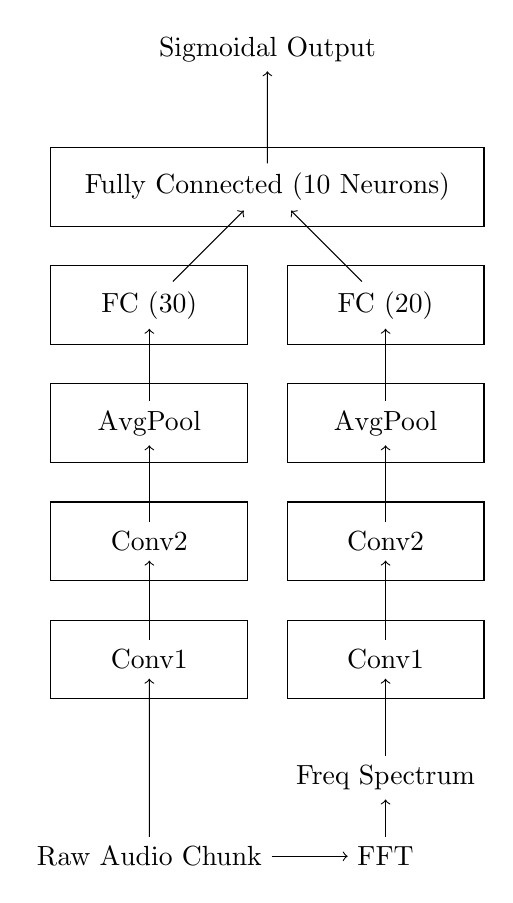
\begin{tikzpicture}
	    \node (output) at (1.25, -.25) {Sigmoidal Output};
	    \draw (-1.5,-1.5) rectangle (4, -2.5) node[pos=.5] (fccombine) {Fully Connected (10 Neurons)};
	    \draw (-1.5,-3) rectangle (1,-4) node[pos=.5] (fcraw) {FC (30)};
	    \draw (1.5,-3) rectangle (4,-4) node[pos=.5] (fcfreq) {FC (20)};
	    \draw (-1.5,-4.5) rectangle (1,-5.5) node[pos=.5] (poolraw) {AvgPool};
	    \draw (1.5,-4.5) rectangle (4,-5.5) node[pos=.5] (poolfreq) {AvgPool};
	    \draw (-1.5,-6) rectangle (1,-7) node[pos=.5] (conv2raw) {Conv2};
	    \draw (1.5,-6) rectangle (4,-7) node[pos=.5] (conv2freq) {Conv2};
	    \draw (-1.5,-7.5) rectangle (1,-8.5) node[pos=.5] (conv1raw) {Conv1};
	    \draw (1.5,-7.5) rectangle (4,-8.5) node[pos=.5] (conv1freq) {Conv1};
	    \node (rawinput) at (-.25, -10.5) {Raw Audio Chunk};
	    \node (fft) at (2.75, -10.5) {FFT};
	    \node (freqinput) at (2.75, -9.5) {Freq Spectrum};
	    
	    \draw[->] (fcraw) -- (fccombine);
	    \draw[->] (fcfreq) -- (fccombine);
	    \draw[->] (poolraw) -- (fcraw);
	    \draw[->] (poolfreq) -- (fcfreq);
	    \draw[->] (conv2raw) -- (poolraw);
	    \draw[->] (conv2freq) -- (poolfreq);
	    \draw[->] (conv1raw) -- (conv2raw);
	    \draw[->] (conv1freq) -- (conv2freq);
	    \draw[->] (rawinput) -- (conv1raw);
	    \draw[->] (rawinput) -- (fft);
	    \draw[->] (fft) -- (freqinput);
	    \draw[->] (freqinput) -- (conv1freq);
	    \draw[->] (fccombine) -- (output);
	\end{tikzpicture}
\end{figure}

\newpage\section{Training}
\textit{(This section satisfies Expectation 4)}

\subsection{Results of Training the ``Raw" Network}

With the original intention of pre-training the two independent subnetworks, we first trained the ``Raw Audio'' CNN by randomly sampling chunks of audio of length 100ms from the files and using these for gradient descent. We split out 80\% of the given data set for training and restricted the remaining 20\% from access by the network in order to utilize it for testing. Because the number of available audio chunks in this test set was so high, it became unrealistic to evaluate network performance on this entire set with each iteration, so it was also sampled. This introduced some variability in the plot of our results, but did not seem to adversely affect our measure of convergence except when the network encountered an occasional outlier in the data. While our network had an error rate of approximately 80\% misclassified pre-training, this was reduced to a mere 7\% in just 4 or 5 epochs. A plot of the MSE against iteration number during training is given below:


\includegraphics[width=\textwidth]{Hans_Net_MSE.PNG}


\subsection{Results of Training the ``FFT" Network}

The convergence of the ``FFT'' CNN during its independent training behaved very similarly to the ``Raw Audio'' network. We repeated the same method, sampling 100ms chunks from the data set for training and testing against files that were set apart from the files used to testing. Also similarly, the network began with a misclassification rate of approximately 80\% and reduced down to misclassifying only approximately 7\% of chunks in just 4 or 5 epochs. A plot of MSE against iteration number is given below:

\includegraphics[width=\textwidth]{Tyler_Net_MSE.PNG}

\subsection{Results of the Joined Network}

Our initial intention was to pretrain the subnetworks described above and use the pretrained weights as the starting point for training of the joint network. After we began training with randomly initialized weights on the full network, we found that the convergence rate was fast enough that pretraining was not necessary. Contrary to the training of the subnetworks, the training of the large network used larger batch sizes, training for 3 hours on a batch of randomly selected chunks that was approximately equal to the size of a full-length audio file from the data set. While our initial attempt at training had little variance, we determined it would be beneficial to reduce the amount of data being used for testing at each iteration to speed up the training process, at the expense of having more variance in the graph of the training error. This training resulted in a relatively consistent rate of error convergence for some period of time before overfitting occurred and the model grew progressively worse. This can be seen in the plot below:

\includegraphics[width=\textwidth]{plotA.png}

Seeing this, we then reset the weights and attempted training again, this time manually implementing an early stop when the model appeared to reach peak performance based on the results from our previous training. This yielded a final error rate of 3.4\% chunks misclassified on test data. The convergence of this manually-stopped training is seen in the plot below:

\includegraphics[width=\textwidth]{plotC.png}

%\subsection{Results of the Post-Processed Data from a Joined Network}


\newpage\section{How Well It Works}
\textit{(This section satisfies Expectation 5)}

Our network was able to achieve 97\% accuracy against the testing data! When we first saw our net getting 90\% accuracy, we assumed that something must be wrong with our net and set out investigating different potential failings. Sadly, because the network processes one chunk of data at a time, a post processing script is required to format the output correctly so it can be opened in Pratt and compared to the human labeled data. Unfortunately, we ran out of time to finish that script, and so we have not had a chance to actually verify the quality of the network in the intended deployment environment.

We should also note that the post processing script will inflate the accuracy of the net even higher. This raises a concern: our goal was to solve the diarization problem, not to achieve high similarity with the human labeled data. Inflating the already high accuracy of the net indicates that the network might have learned to model human labeling behavior in addition to diarization, meaning that we might have had better accuracy solving the diarization problem if we had stopped training earlier.

%\subsection{Results and Commentary}


\newpage\section{Concluding Remarks and Future Work}
\textit{(This section satisfies Expectation 6)}

While we feel excited about the roughly 100 hours our group put into this assignment, we also acknowledge we didn't achieve everything and are anxious to try the following overarching ideas in future:

\begin{itemize}
\item[Dropout Learning] This, more than perhaps any other feature, was a key aspect of our training we wanted to attempt. Our set of training data is large, so we are cautiously optimistic that we won't need to worry about over-fitting. Yet because our error is so low, one does wonder.
\item[Non-ReLU Functions] Another key idea we wished to try was using non ReLU functions in our net, trying instead soft-ReLUs or even other totally non-linear functions, such as arctan.
\item[RBMs] We initially wanted to prime our network with a Restricted Boltzmann Machines or even utilize it as an input layer to the function. We believed that, as Geoff Hinton has suggested, a network that can ``dream about'' the types of speech occurring in our data set, then it can recognize that speech. We hoped to give the network a chance to develop some underlying distribution to represent the different types, timbres, and frequencies of speech, as well as of background noise, so that it could more easily distinguish them. This was a feature we were unable to implement given the time constraints, but we still think it would improve the network.
\end{itemize}

Overall, however, we are pleased with this project and content with the semester. We think that the key aspects which we learned are that Neural Nets are not a one-size-fits-all solution to every problem, many problems/bugs encountered within neural net coding are often subtle, and that TensorFlow is the leading neural net library for a reason - it's incredibly powerful.

Once again, thank you Dr. Moon for a wonderful semester. Enjoy your holiday season!

% Ideas for future work:
% * Dropout learning
% * Cross entropy as error function
% * Wanted to see how functions other than RELU performed



\newpage\section{Appendix: Code}
\textit{(This section satisfies Expectation 7)}








%----------------------------------------------------------------------------------------

\end{document}